%1521001##1##.tex
\documentclass[12pt,letterpaper]{article}
\usepackage{mathptmx}
\usepackage[margin=1in]{geometry}

\usepackage{setspace}
\singlespacing
  
\usepackage{amssymb,latexsym}
\usepackage[round,sort]{natbib}
\usepackage{fancyhdr}
\usepackage{lastpage}
\usepackage{graphicx}
\graphicspath{ {qe2/} }

% Bold Table and Figure captions
\usepackage{caption}
\captionsetup{figurename=FIGURE}
\captionsetup{tablename=TABLE}
\captionsetup[figure]{labelfont=bf}
\captionsetup[table]{labelfont=bf}
  
% Turns off all section numbering
\setcounter{secnumdepth}{0} 

  % Places all tables at end of document and creates AOM-style table-here placeholders
  \usepackage[nolists]{endfloat} % Places all figures and charts at end of manuscript and adds 'insert table x about here' lines.
  \renewcommand{\figureplace}{
    \begin{center}
    \begin{singlespace}
    ------------------------------------\\
    Insert \figurename \ \thepostfig\ about here.\\
    ------------------------------------
    \end{singlespace}
    \end{center}}
  \renewcommand{\tableplace}{%
    \begin{center}
    \begin{singlespace}
    ------------------------------------\\
    Insert \tablename \ \theposttbl\ about here.\\
    ------------------------------------
    \end{singlespace}
    \end{center}}

  \usepackage{titlesec}
   \titleformat{\title}
       {\filcenter\normalfont\bfseries\uppercase}{\thetitle}{1em}{}
  \titleformat{\section}
    {\filcenter\normalfont\bfseries\uppercase}{\thesection}{1em}{}
  \titleformat{\subsection}
    {\normalfont\bfseries}{\thesubsection}{1em}{}
  \titleformat{\subsubsection}[runin]
   {\normalfont\bfseries\slshape}{\thesubsubsection}{1em}{\hspace*{\parindent}}
       
\usepackage{tabu}
\usepackage{textcomp}
\usepackage{listings}
\usepackage{hyperref}
\usepackage{verbatim}
\usepackage{tabu}
\hypersetup{
    colorlinks=true,
    linkcolor=blue,
    filecolor=cyan,      
    urlcolor=cyan,
    citecolor=blue,
}

\usepackage{etoolbox}

\makeatletter

% Patch case where name and year are separated by aysep
\patchcmd{\NAT@citex}
  {\@citea\NAT@hyper@{%
     \NAT@nmfmt{\NAT@nm}%
     \hyper@natlinkbreak{\NAT@aysep\NAT@spacechar}{\@citeb\@extra@b@citeb}%
     \NAT@date}}
  {\@citea\NAT@nmfmt{\NAT@nm}%
   \NAT@aysep\NAT@spacechar\NAT@hyper@{\NAT@date}}{}{}

% Patch case where name and year are separated by opening bracket
\patchcmd{\NAT@citex}
  {\@citea\NAT@hyper@{%
     \NAT@nmfmt{\NAT@nm}%
     \hyper@natlinkbreak{\NAT@spacechar\NAT@@open\if*#1*\else#1\NAT@spacechar\fi}%
       {\@citeb\@extra@b@citeb}%
     \NAT@date}}
  {\@citea\NAT@nmfmt{\NAT@nm}%
   \NAT@spacechar\NAT@@open\if*#1*\else#1\NAT@spacechar\fi\NAT@hyper@{\NAT@date}}
  {}{}

\lstset{
basicstyle=\ttfamily,
columns=flexible,
breaklines=true
}
\newenvironment{hypothesis}{
  	\itshape
  	\leftskip=\parindent \rightskip=\parindent
  	\noindent\ignorespaces}

\fancypagestyle{plain}{
  \renewcommand{\headrulewidth}{0pt}
  \fancyhf{}
}	


\begin{document}
\title{Organizational Learning and Human Capital: Similarities and Tensions}
\date{}
\maketitle

\begin{abstract} 
\normalsize 
We apply a formal model to understand the effects of the relative learning rates of embedded agents and the institutional field on organizational outcomes. 
\end{abstract}


{\textbf{Keywords:} \\\indent Embedded Agency}

\newpage
\pagestyle{fancy}
\fancyhf{}
\lhead{Organizational Learning and Human Capital}
\rhead{\thepage}

\begin{center}
\textbf{Title: Sub-title}
\end{center}


Today?s organizations increasingly rely on intangible assets such as human capital to gain a competitive advantage (e.g., Barney, 1991)
some of the linkages between micro and macro areas are already occurring, for example in the domain of human capital and strategy (e.g. Coff & Kryscynski, 2011; Ployhart & Moliterno, 2011. The idea of ?microfoundations? can be traced to historical tensions between micro and macro disciplines in the social sciences. The central tension has been whether explanations of individual and collective or societal outcomes should focus on the individual or societal and cultural level (Udehn, 2001)
Similar intuition has been echoed and further reinforced in some of the most highly cited and seminal work in strategic management over the past two decades, specifically arguing that individual-level considerations simply are not relevant for strategy and firm-level outcomes (see Henderson & Cock- burn, 1994; Kogut & Zander, 1992, 1996; Nahapiet & Ghoshal, 1998; Spender, 1996). This literature places an emphasis on macro factors such as firm-level knowledge and competencies, social capital, networks, and other collective constructs. Henderson and Cockburn (1994) assume in their highly cited empirical analy- sis of organizational competencies that individuals are homogeneous, and thus they ascribe performance variance to collective-level routines and practices. The microfoundations literature and movement, then, can be seen as a reaction to an over-emphasis on collective factors, as well as the seeming disregard for individual-level and social interactional considerations in explaining organiz- ational outcomes.


To provide another specific example, foundational and highly cited macro concepts such as firm-level ?absorptive capacity? (Cohen & Levinthal, 1990) can be directly traced to equivalent, individual-level concepts in psychology. Specifically, the oldest citations in Cohen and Levinthal?s influential article are to behavioral psychology and learning theory related to individual knowl- edge acquisition based on experience, stimulus, and repetition (e.g. Bower & Hilgard, 1981; Ellis, 1965; Estes, 1970; Harlow, 1949). These individual-level concepts were applied directly to the firm and coined as ?absorptive capacity?. While the concept of absorptive capacity, of course, is important, the paper itself did not explicitly theorize how the concept might need to change and evolve when applied to the organization as a unitary actor (though, subsequent efforts have been made in this direction). Other examples of the one-to-one application of concepts from micro to macro include cognition and learning by association and analogy (e.g. Gavetti, 2012; Gavetti, Levinthal, & Rivkin, 2005).



From an organizational learning perspective, recipient firms are likely to be concerned with two issues related to ability to learn: first, whether they can effectively understand and apply the spilled over knowledge; and second, the additional complementary oppor- tunities for learning from the originator. If the knowledge is in one of the areas of specialization of the recipient firm, the recipient?s absorptive capacity (Cohen and Levinthal, 1990) for the spilled over knowledge as well as for complementary knowledge is likely to be high. The absorptive capacity of the firm for external technological knowledge is dependent to a significant extent on the degree of its knowledge in a particular technological field (Schoenmakers and Duysters, 2006). Further, the develop- ment and accumulation of tacit knowledge (Polanyi, 1966) related to the technology is also dependent on specialization (Enright, 1991). Thus a recipient with greater speciali- zation will possess well-developed internal mechanisms for understanding and exploiting spillover knowledge.
 their macro approach, and assumptions about the homogeneity of human capital, by arguing that stars cannot be a source of sustainable advantage as they appropriate their marginal rents. In other words, the reason that some have focused directly on collective capability is that information about the capability of particu- lar individuals (if markets are relatively efficient), such as stars, is likely to be widely available and thus these individuals are perhaps able to appro- priate any rents associated with their abilities.
Our theory also links work in the knowledge- based view (e.g., Grant, 1996; Kogut and Zander, 1992) with work on strategic human capital (e.g., Campbell, Coff, and Kryscynski, 2012; Coff, 1997). The literature has long held that routines are ?repos- itories and carriers of knowledge? (Hodgson, 2008: 25). We show that organizational memory is a nat- ural outcome of the process through which routines emerge, and knowledge is thus not only in the minds of (and embodied in the habits of) individuals, but also in the connections between individuals. Con- sider employee turnover. We  nd that the exit of one individual does not undermine the performance of the routine. Even if the departing individual does not explicitly transfer his or her knowledge to the replacement person, the routinized behavior of the remaining individuals will lead him or her to select a task approach that resembles his or her predeces- sor. Thus, the knowledge embodied in the connec- tions between individuals has the properties of tacit knowledge. Once formed, such knowledge is not subject to expropriation by individuals ? it is inher- ently the property of the organization.

Coff and Kryscynski (2011) explored human capital-based competitive advan- tage and, while their focus was clearly within the firm, they did note that when causal ambiguity is derived from tacit knowledge it creates problems of imitation for both people within the firm and for competitors.
Characteristics, Base discipline, level of analysis, key assumptions

Organizational Learning


Human Capital

\section{Background}
 \cite{Scott1995} visualized institutional fields as a community of organizations that partakes of a common meaning system and whose participants interact more frequently and fatefully with one another than with actors outside the field. 
 
\section{Model}

We develop a simple model consisting of two players who participate in a repeated game of matching \footnote{I am grateful to Phanish Puranam for having introduced me to this model of reinforcement learning during a workshop at the Indian Institute of Science on 16th December, 2016. His definitions and code have been extensively reused in this work.}. The payoffs are captured by the matrix in Table ~\ref{payoffmatrix}

\begin{table}
\begin{centering}
\caption {Payoff Matrix}
\label{payoffmatrix}
{\tabulinesep=1.4mm
\begin{tabu}{|c|c|c|}
\hline
&$choice_F(t) = 0$&$choice_F(t) = 1$\\\hline
$choice_A(t) = 0$&$[payoff_F(t),payoff_A(t)]=[1,1]$&$[payoff_F(t),payoff_A(t)]=[0,0]$\\\hline
$choice_A(t) = 1$&$[payoff_F(t),payoff_A(t)]=[0,0]$&$[payoff_F(t),payoff_A(t)]=[1,1]$\\\hline
\end{tabu}}

\end{centering}
\end{table} 

To help improve the intuition in the analysis, we define a few categories. 

\subsection{Field Start Position}
The Field Start Position is a characterization of the choice preference of the institutional field at the start of the interaction. 
\subsubsection{The third level section}
We do so since the scale is symmetric across the Center (C), any initial mapping of Left (L) and Left of Center (LC) can be mapped onto an equivalent Right (R) or Right of Center (RC) configuration. 

\begin{figure}[h]
\begin{centering}
  \caption{}
  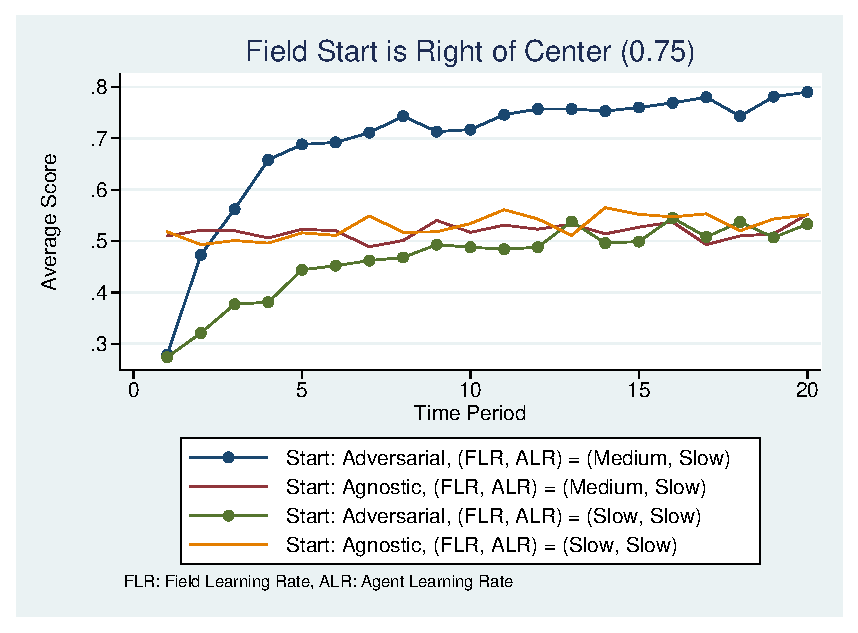
\includegraphics[width=\textwidth]{frcmedium3a}
  \label{fig:3a}
\end{centering}
\end{figure}

\section{Discussion}
Having laid out the formal model and having described the assumptions and classifications made in the previous section, we now consider if the model described above is a reasonable abstraction of the phenomenon that we wish to theorize upon. 

\section{Interpretation of Model Results}
\subsection{On the topic of the general hypotheses}
 Figure ~\ref{fig:3a} lays out the average score charts for four agent-field combinations while enforcing the field to start in Right of Center (this is the same as saying $p_{0,F}^0 = 0.75$). 
\subsubsection{Leading into H1a}
We do so since the scale is symmetric across the Center (C), any initial mapping 

\begin{hypothesis}
{Hypothesis 1a: When the institutional field is open to influence, slow learning adversarial agents will raise overall performance higher than slow learning agents with a neutral orientation\\}
\end{hypothesis}

\subsubsection{Leading into H2a}
This trend is confirmed further in Figure ~\ref{fig:3a} where the learning rates of agents are increased even further to \textquotesingle Fast\textquotesingle .

\begin{hypothesis}
{Hypothesis 2a: For the same initial outcome preferences,  the overall performance score varies curvilinearly with difference in the rates of learning of the agent and the institutional field\\}
\end{hypothesis}

\section{Limitations and Future Work}
The formal computational modeling approach to theorizing organizational phenomena comes across as being both valuable and challenging simultaneously. 


\section{Conclusion}
We started out attempting to improve our understanding of the mechanisms behind the embedded agent - institutional field engagement. 

\begin{comment}
\section{Acknowledgements}
All mistakes made here are completely mine. 
\end{comment}

\newpage
\begin{singlespace}
\bibliography{/Users/aiyenggar/code/bibliography/aiyenggar} 
\bibliographystyle{ai-amjlike}
\end{singlespace}

\newpage
\appendix
\begin{singlespace}
\section{APPENDIX A: Simulation Code}
\lstinputlisting{qe2/matchingEmbeddedAgency.py}
\end{singlespace}

\end{document}
